\documentclass[11]{article}
\usepackage{amsthm, amssymb, amsmath,verbatim}
\usepackage[margin=1in]{geometry}
\usepackage{enumerate}
\usepackage{enumitem}
\usepackage{graphicx}

\newtheorem*{claim}{Claim}
\newtheorem{ques}{Question}

\title{CSE 150 Homework 2}
\date{Fall 2018}
\author{Pedro Sousa Meireles}
\begin{document}

\maketitle
\section{Variable Elimination Algorithm}
\begin{enumerate}[label=(\alph*)]
\item{\textbf{Computing using variable elimination}}

Eliminating S:

\begin{table}[htp]
\centering
\begin{tabular}{c|c}
F & $f_3'(F)$ \\ \hline
0 & 0.01       \\ \hline
1 & 0.9       
\end{tabular}
\end{table}

Eliminating R:

\begin{table}[htp]
\centering
\begin{tabular}{c|c}
L & $f_5'(L)$ \\ \hline
0 & 0.01       \\ \hline
1 & 0.75      
\end{tabular}
\end{table}

Eliminating L:

$$f_6(A)=\sum_l f_5'(L=l) \cdot f_4(A,L=l)$$

Eliminating L costs 1 addition and 2 products per different A, making 2 additions and 4 products.

\begin{table}[htp]
\centering
\begin{tabular}{c|c}
A & $f_6(A)$   \\ \hline
0 & 0.01074 \\ \hline
1 & 0.6612 
\end{tabular}
\end{table}

Eliminating A:

$$f_7(T,F)=\sum_a f_2(T,F,A=a) \cdot f_6(A=a)$$

Eliminating A costs 1 addition and 2 products per different (T,F), making 4 additions and 8 products.

\begin{table}[htp]
\centering
\begin{tabular}{c|c|c}
T & F & $f_7(T,F)$  \\ \hline
0 & 0 & 0.010805046 \\ \hline
0 & 1 & 0.6546954   \\ \hline
1 & 0 & 0.563631    \\ \hline
1 & 1 & 0.33597    
\end{tabular}
\end{table}
\pagebreak

Eliminating F:

$$f_7(T)=\sum_a f_1(F=f) \cdot f_7(T,F=f) \cdot f_3'(F=f)$$

Eliminating F costs 1 addition and 4 products per different T, making 2 additions and 8 products.

\begin{table}[htp]
\centering
\begin{tabular}{c|c}
T & $f_7(T)$      \\ \hline
0 & 0.00599922865 \\ \hline
1 & 0.0086036769 
\end{tabular}
\end{table}

Combining T factors:

$$f_8(T)=f_0(T) \cdot f_7(T)$$

Combining T factors costs 0 additions and 1 products per different T, making 0 additions and 2 products.

\begin{table}[htp]
\centering
\begin{tabular}{c|c}
T & $f_8(T)$       \\ \hline
0 & 0.00587924408  \\ \hline
1 & 0.000172073538
\end{tabular}
\end{table}

$$P(T=0|S=1,R=1)=\frac{f_8(T=0)}{f_8(T=0)+f_8(T=1)}=0.97156$$
$$P(T=1|S=1,R=1)=\frac{f_8(T=1)}{f_8(T=0)+f_8(T=1)}=0.02843$$

\item{\textbf{Counting calculations used by the variable elimination algorithm}}

\begin{table}[htp]
\centering
\begin{tabular}{|c|c|c|c|}
\hline
\textbf{Phase of algorithm}   & \textbf{\# multiplications} & \textbf{\# additions} & \textbf{\# divisions} \\ \hline
Eliminate S (evidence)        & 0                           & 0                     & 0                     \\ \hline
Eliminate R (evidence)        & 0                           & 0                     & 0                     \\ \hline
Eliminate L                   & 4                           & 2                     & 0                     \\ \hline
Eliminate A                   & 8                           & 4                     & 0                     \\ \hline
Eliminate F                   & 8                           & 2                     & 0                     \\ \hline
Combine T factors             & 2                           & 0                     & 0                     \\ \hline
Normalize distribution over T & 0                           & 1                     & 2                     \\ \hline
\textbf{Total}                & 22                          & 9                     & 2                     \\ \hline
\end{tabular}
\end{table}
\pagebreak
\item{\textbf{Counting calculations used by the enumeration algorithm}}
\begin{align*}
& P(T=0,S=1,R=1) =\sum_a \sum_f \sum_l P(A=a,F=f,L=l,R=1,S=1,T=0)\\
&= \sum_a \sum_f \sum_l P(T=0) \cdot P(F=f) \cdot P(S=1|F=f) \cdot P(A=a|T=0,F=f) \cdot P(L=l|A=a) \cdot P(R=1|L=l)
\end{align*}

\begin{align*}
& P(T=1,S=1,R=1) =\sum_a \sum_f \sum_l P(A=a,F=f,L=l,R=1,S=1,T=1)\\
&= \sum_a \sum_f \sum_l P(T=0) \cdot P(F=f) \cdot P(S=1|F=f) \cdot P(A=a|T=1,F=f) \cdot P(L=l|A=a) \cdot P(R=1|L=l)
\end{align*}

The sums have 8 terms, which makes 7 additions each, and each term is a product of 6 probabilities, what accounts 5 multiplications per term, which makes 7 additions and 40 multiplications each.

\begin{table}[htp]
\centering
\begin{tabular}{|c|c|c|c|}
\hline
\textbf{Phase of algorithm}   & \textbf{\# multiplications} & \textbf{\# additions} & \textbf{\# divisions} \\ \hline
Compute $P(T=0,S=1,R=1)$      & 40                         & 7                    & 0                    \\ \hline
Compute $P(T=1,S=1,R=1)$      & 40                         & 7                    & 0                    \\ \hline
Normalize distribution over T & 0                          & 1                    & 2                    \\ \hline
\textbf{Total}                & 80                         & 15                   & 2                    \\ \hline
\end{tabular}
\end{table}
\end{enumerate}
\pagebreak

\section{To be, or not to be, a polytree: that is the question}

\begin{figure}[htp]
  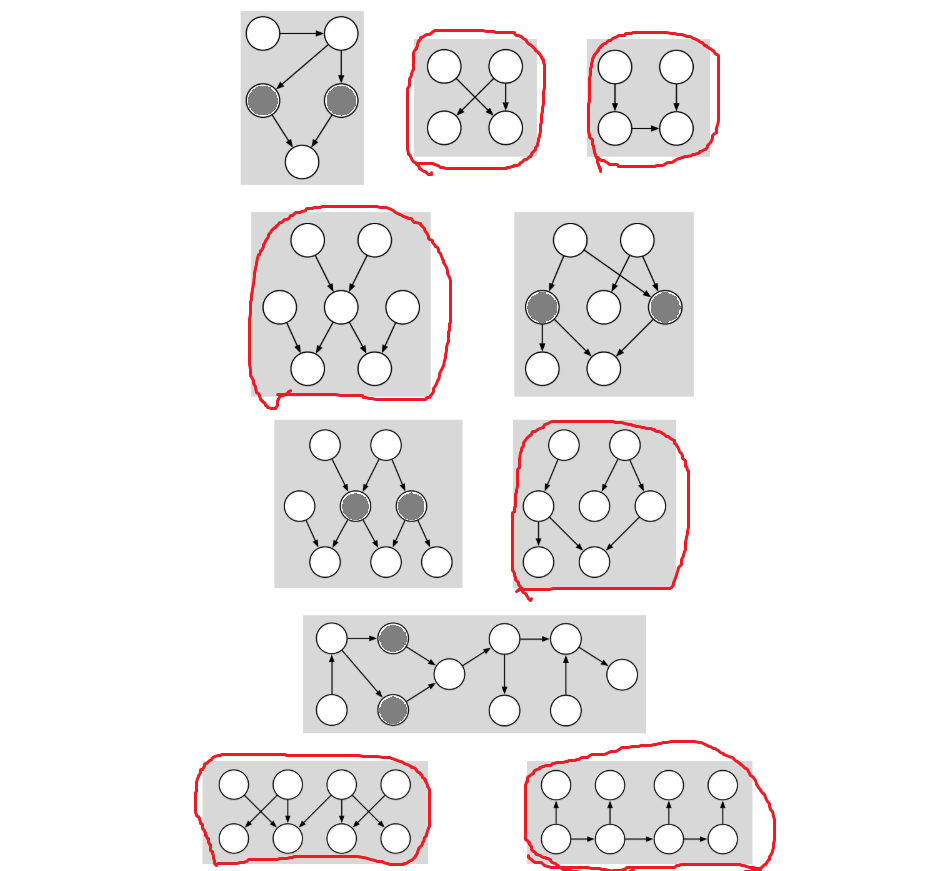
\includegraphics[width=\linewidth]{Polytrees.png}
\end{figure}
\pagebreak

\section{Node clustering}

\begin{table}[htp]
\centering
\begin{tabular}{|c|c|c|c|c|c|c|c|}
\hline
$Y_1$ & $Y_2$ & $Y_3$ & $Y$ & $P(Y|X=0)$ & $P(Y|X=1)$ & $P(Z_1=1|Y)$ & $P(Z_2=1|Y)$ \\ \hline
0     & 0     & 0     & 1   & 0.0525     & 0.14625    & 0.8          & 0.2          \\ \hline
1     & 0     & 0     & 2   & 0.2975     & 0.04875    & 0.7          & 0.3          \\ \hline
0     & 1     & 0     & 3   & 0.0225     & 0.07875    & 0.6          & 0.4          \\ \hline
0     & 0     & 1     & 4   & 0.525      & 0.34125    & 0.5          & 0.5          \\ \hline
1     & 1     & 0     & 5   & 0.1275     & 0.02625    & 0.4          & 0.6          \\ \hline
1     & 0     & 1     & 6   & 0.2975     & 0.11375    & 0.3          & 0.7          \\ \hline
0     & 1     & 1     & 7   & 0.0225     & 0.18375    & 0.2          & 0.8          \\ \hline
1     & 1     & 1     & 8   & 0.1275     & 0.06125    & 0.1          & 0.9          \\ \hline
\end{tabular}
\end{table}
\pagebreak


\section{Maximum likelihood estimation for an n-sided die}
\begin{enumerate}[label=(\alph*)]
\item{\textbf{Log-likelihood}}
\begin{align*}
likelihood(p) &= P({x^{(1)}, ..., x^{(T)}})\\
&= \prod_{t=1}^T P(X=k) \\
&= p_1^{C_1} \cdot p_2^{C_2} \cdot ... \cdot p_n^{C_n}
\end{align*}

Applying log in the equation and separating the log of a productory in a sum of logs:
\begin{align*}
L(p) &= C_1 \cdot p_1 + C_2 \cdot p_2 + ... + C_n \cdot p_n \\
&= \sum_{k=1}^n C_k \cdot p_k
\end{align*}

\item{\textbf{KL distance}}

\begin{align*}
KL(q,p) &= \sum_k q_k \cdot log \left( \frac{q_k}{p_k} \right)\\
&= \sum_k q_k \cdot (log(q_k) - log(p_k))\\
&= \sum_k q_k \cdot log(q_k) - \sum_k \frac{C_k \cdot log(p_k)}{T}\\
&= \sum_k q_k \cdot log(q_k) - \frac{\sum_k C_k \cdot log(p_k)}{T}\\
&= \sum_k q_k \cdot log(q_k) - \frac{L(p)}{T}
\end{align*}

Given a set of tosses, the left term is constant, which means the value of the difference varies only with $L(p)$ variation. So, maximizing $L(p)$ is equivalent to minimizing the KL distance.

\item{\textbf{Maximum likelihood estimation}}

In the last item we proved that maximizing $L(p)$ is equivalent to minimizing $KL(q,p)$. Also, in homework problem 1.6b, we proved that $KL(p,q) \geq 0$, with equality only when $p = q$. So, to maximize $L(p)$, we have to make $p_k=q_k$. Then, $p_k = \frac{C_k}{T}$.
\end{enumerate}

\end{document} 